\section{Umsetzung des realen Clusters}\label{sec:aufbauCluster}

\citeauthor{zhang2016} haben im Rahmen ihrer gesamten Forschungsarbeit die Open"=Source"=Plattform Hadoop"=Benchmark entwickelt und auf Github zur Verfügung gestellt.\footnote{\url{https://github.com/Spirals-Team/hadoop-benchmark}}
Sie wurde speziell zum Einsatz in der Forschung erstellt und kann jederzeit an die eigenen Bedürfnisse angepasst werden.
Auf Basis dieser Plattform und der enthaltenen Benchmarks wurde das reale Cluster für diese Masterarbeit aufgebaut.

\subsection{Plattform Hadoop"=Benchmark}\label{sec:hadoopBenchmark}

Die Plattform ist in mehrere Szenarien unterteilt, darunter ein Hadoop in der Version 2.7.1 ohne Änderungen und ein darauf basierendes Szenario mit der Selfbalancing"=Komponente.
Hadoop"=Benchmark basiert auf der Software \emph{Docker}\footnote{\url{https://www.docker.com/}} und dem dazugehörigen Tool \emph{Docker Machine}, um damit mit wenigen Befehlen ein Hadoop"=Cluster aufbauen zu können.
Mit \emph{Graphite}\footnote{\url{https://graphiteapp.org/}} ist zudem ein Monitoring"=Tool enthalten, mit dem die Systemwerte wie CPU- oder Speicher"=Auslastung des Clusters überwacht und analysiert werden kann.

\begin{figure}
    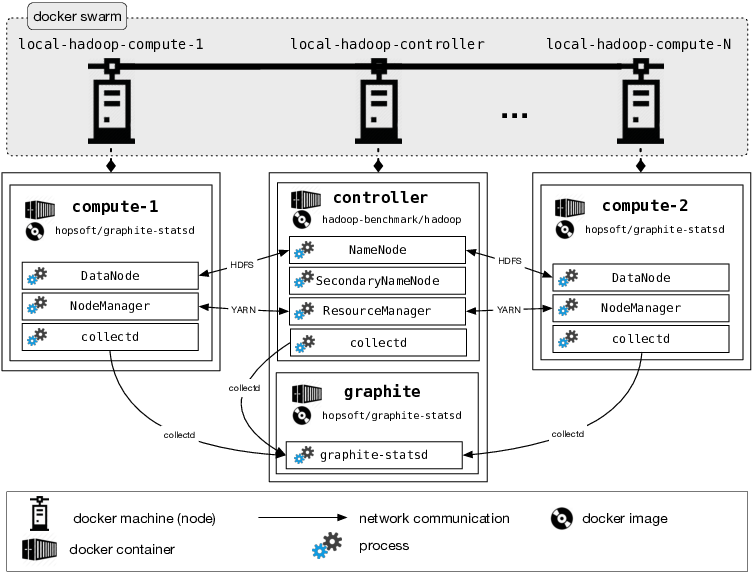
\includegraphics{./images/hadoopBenchmarkArch.png}
    \caption[High"=Level"=Architektur von Hadoop"=Benchmark]
    {High"=Level"=Architektur von Hadoop"=Benchmark.
        Entnommen aus \cite{abb:hadoopBenchmarkArch}.}
    \label{fig:hadoopBenchmarkArchitecture}
\end{figure}

\autoref{fig:hadoopBenchmarkArchitecture} zeigt die grundlegende Architektur der Plattform, die mithilfe eines Docker"=Swarms auf mehreren \emph{Docker Machines} ein Cluster erstellt, auf denen dann in den Docker"=Containern das eigentliche Hadoop"=Cluster ausgeführt wird.
In Hadoop"=Benchmark werden mithilfe von Docker"=Machine und VirtualBox\footnote{\url{https://www.virtualbox.org/}} virtuelle Maschinen erstellt, die mit dem  Betriebssystem \emph{Boot2Docker} ausgestattet sind.
Boot2Docker ist eine leichtgewichtige Linux"=Distribution, auf der Docker bereits vorinstalliert ist \cite{DockerMachineGettingStartedVm}.
Jeder Hadoop"=Container enthält zudem das Tool \emph{collectd}\footnote{\url{https://collectd.org/}}, was das Monitoring des Containers auf Systemebene übernimmt und die Daten an den Graphite"=Container übermittelt.
Dadurch wird es möglich, eine beliebige Anzahl an voneinander unabhängigen Nodes auf einem physischen Computer ausführen zu können.
Auch ist es möglich, den Docker"=Machines einen beliebig großen Arbeitsspeicher zur Verfügung zu stellen.

Die Plattform Hadoop"=Benchmark enthält zudem einige Benchmark"=Anwendungen:

\begin{itemize}
    \item Hadoop Mapreduce Examples
    \item Intel HiBench\footnote{\url{https://github.com/intel-hadoop/HiBench}}
    \item \ac{SWIM} \footnote{\url{https://github.com/SWIMProjectUCB/SWIM}}
\end{itemize}

Eine Besonderheit bildet der SWIM"=Benchmark, welcher sehr Ressourcenintensiv ist und daher auf einem \emph{Single Node Cluster}, also einem kompletten Hadoop"=Cluster auf nur einem Computer, sehr zeitintensiv sein kann.
Der Intel HiBench"=Benchmark besteht aus Kategorien wie \emph{Machine Learning} oder Graphen, welche wiederum aus einen oder mehreren \emph{Workloads} bestehen, welche entsprechende Anwendungen bzw. Algorithmen auf dem Hadoop"=Cluster ausführen.
Einige der Hibench"=Workloads basieren auf den Mapreduce Examples, welche wiederum voneinander unabhängige Beispielanwendungen für Hadoop darstellen.

\subsection{In dieser Fallstudie verwendetes Setup}\label{sec:clusterFallstudie}

Da die Plattform Hadoop"=Benchmark mithilfe von Docker auf einem physischen PC sehr einfach ein komplettes Hadoop"=Cluster ausführen kann, wurde die Plattform für diese Fallstudie als Basis genutzt.
Da Docker und Hadoop vor allem für den Einsatz in einer Linux"=Umgebung entwickelt wurden, werden für die Fallstudie zwei Computer genutzt, auf denen das Cluster wahlweise auf einem oder auf beiden Hosts ausgeführt werden kann.
Zudem wird auf einem Host eine VM mit Windows 10 ausgeführt, das zum Ausführen des .NET"=Frameworks bzw. \sS benötigt wird.
Beide zum Einsatz kommenden Hosts sind jeweils mit einem Intel Core i5"=4570 @ 3,2 GHz x 4, 16 GB Arbeitsspeicher sowie einer SSD ausgestattet, auf der Ubuntu 16.04 LTS installiert ist.
Die Verbindung von Windows zu Linux auf beiden Hosts wird mithilfe von SSH"=Verbindungen umgesetzt.

\begin{figure}
    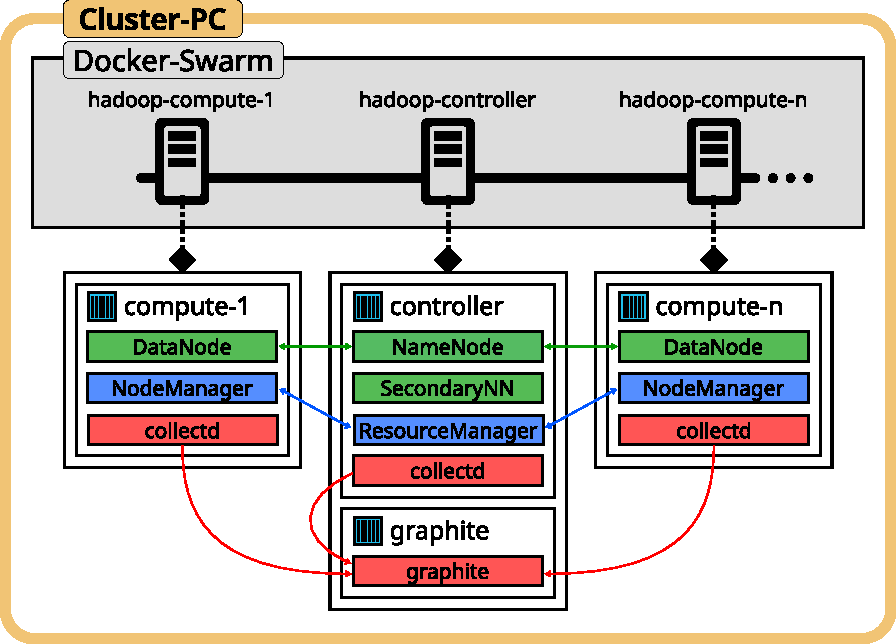
\includegraphics{./images/caseStudyHadoopSetup.pdf}
    \caption[In der Fallstudie verwendetes Cluster"=Setup]
    {In der Fallstudie verwendetes Cluster"=Setup.
        Grün: \ac{HDFS}, Blau: YARN, Rot: Graphite.}
    \label{fig:caseStudyHadoopSetup}
\end{figure}

Die beiden Abbildungen \autoref{fig:hadoopBenchmarkArchitecture} und \autoref{fig:caseStudyHadoopSetup} zeigen bereits den großen Hauptunterschied zwischen der Plattform und dem hier verwendeten Cluster"=Setup.
Da durch die Nutzung von virtuellen Maschinen ein zusätzlicher Ressourcenbedarf entsteht, wird im hier verwendeten Setup darauf verzichtet.
Durch die Ausführung der Docker"=Container des Hadoop"=Clusters direkt auf dem Host stehen dem Cluster mehr Ressourcen zur Verfügung.
Zudem wird es mithilfe von von \emph{Docker Swarm} so ermöglicht, das Hadoop"=Cluster auf beiden Hosts auszuführen.
Im konkreten Setup werden dabei Graphite, der Hadoop"=Controller sowie vier Hadoop"=Nodes auf dem Host1, sowie zwei weitere, optionale Nodes auf Host2 ausgeführt.
Weitere Anpassungen des verwendeten Setups bestehen \uA darin, dass der \ac{TLS} von Hadoop ebenfalls gestartet wird.
Zudem wurden einige Einstellungen von Hadoop so angepasst, dass defekte Nodes schneller erkannt werden.

Zum Ausführen der Windows"=VM auf Host2 wird VirtualBox 5.2 verwendet.
Zum Abrufen von Daten mithilfe der REST"=API von Hadoop über die SSH"=Verbindungen wird \emph{curl}\footnote{\url{https://curl.haxx.se/}} genutzt.
Zum Ausführen des Hadoop"=Clusters wird Docker in der Version 18.03 CE genutzt.

Um die in dieser Fallstudie benötigten Befehle einfach ausführen zu können, wurden zwei eigene Scripte erstellt, welche zum Teil auf den bestehenden Scripten der Plattform aufbauen.
Das Setup"=Script dient für folgende Zwecke:

\begin{itemize}
    \item Starten und Beenden des Clusters
    \item Starten und Beenden einzelner Hadoop"=Nodes
    \item Hinzufügen und Entfernen der Netzwerkverbindung des Docker"=Containers eines Hadoop"=Nodes
    \item Ausführen von eigenen Befehlen auf dem Docker"=Container des Hadoop"=Controllers
    \item Erstellen des Hadoop"=Docker"=Images
\end{itemize}

Das zweite erstellte Script dient ausschließlich zum Starten der Benchmarks.
Dazu werden die in der Plattform bereits enthaltenen Start"=Scripte aufgerufen, die für das konkrete Setup angepasst wurden.
